\chapter*{APPENDIX A: SYSTEM USER INTERFACE DEMONSTRATION}
\addcontentsline{toc}{chapter}{APPENDIX A: SYSTEM USER INTERFACE DEMONSTRATION}

\section*{A.1 Interactive Operations Center Command View}
Figure~A.1 presents the complete layout of the CivicTwin Operations Center dashboard, showing the real-time interaction between the top-level KPI metrics, the left control sidebar, and the central Leaflet vector GIS map.

\begin{figure}[h!]
\centering
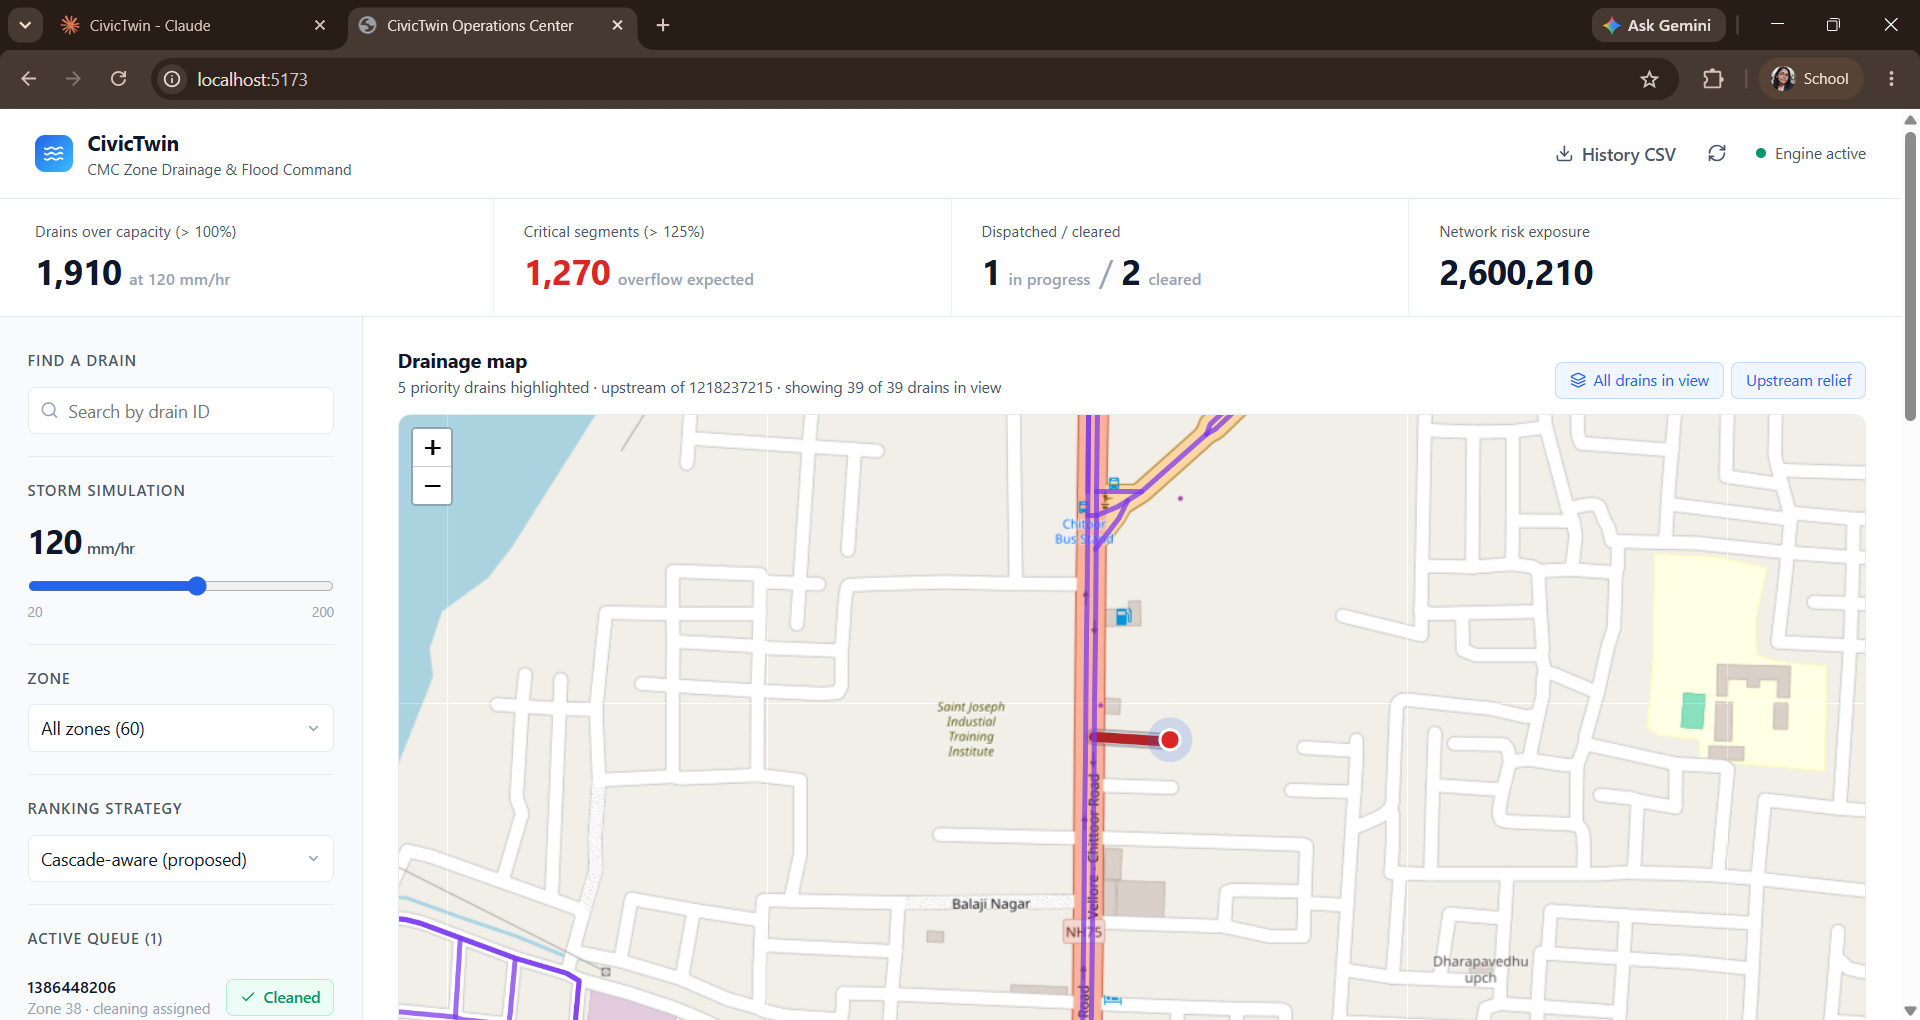
\includegraphics[width=0.98\textwidth]{figures/ui_map_dashboard.png}
\caption*{Fig. A.1 Full CivicTwin Operations Center Interface Showing GIS Map and Live KPI Counters}
\end{figure}

\section*{A.2 Priority Dispatch Queue and Structural Overload Metrics}
Figure~A.2 shows the priority dispatch queue where municipal operators inspect conduit IDs, physical structures, surveyed silt levels, and intuitive capacity utilization bars with diagonal striped overflow patterns.

\begin{figure}[h!]
\centering
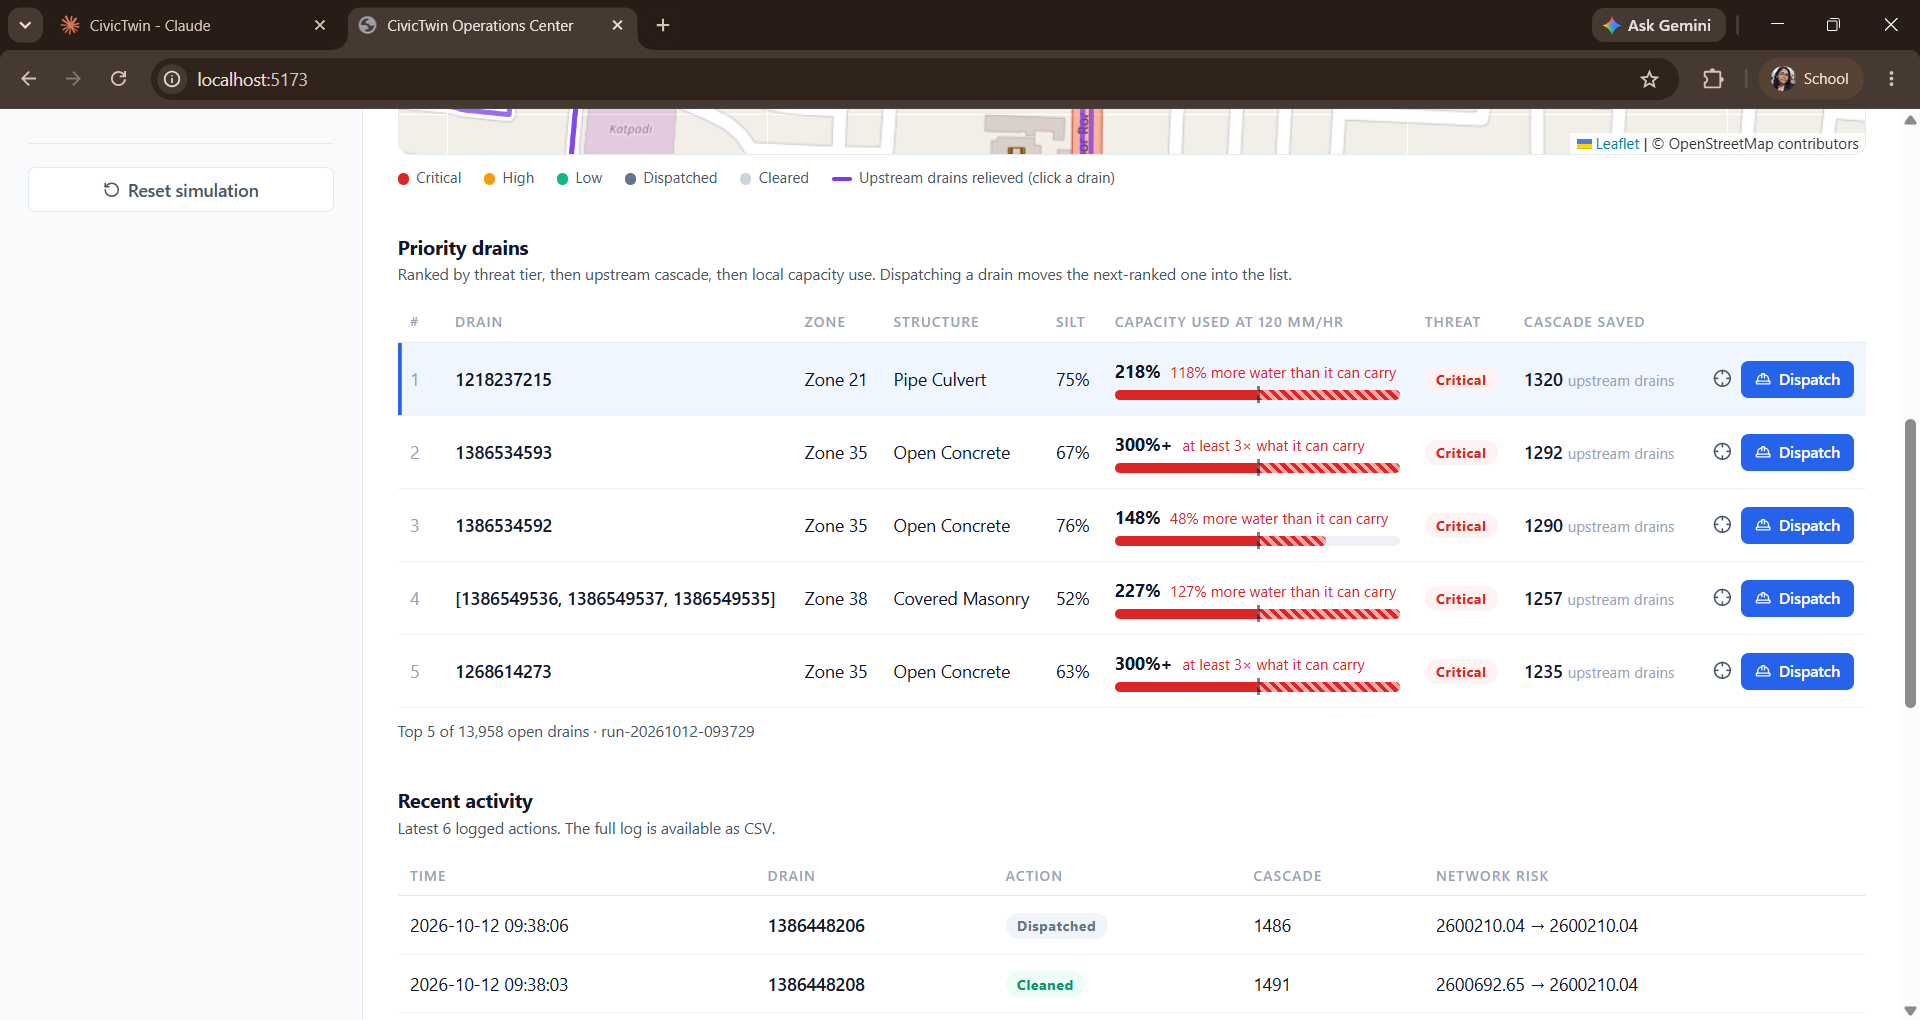
\includegraphics[width=0.98\textwidth]{figures/ui_priority_table.png}
\caption*{Fig. A.2 Priority Drains Table Showing Surcharge Ratios, Upstream Cascade Reachability, and Dispatch Actions}
\end{figure}

\section*{A.3 Operational Activity Audit Trail and Interpretation Guidelines}
Figure~A.3 illustrates the recent activity audit logging panel, showing immutable records of field dispatches, cleaning completions, upstream cascade reliefs, and quantitative network risk deltas.

\begin{figure}[h!]
\centering
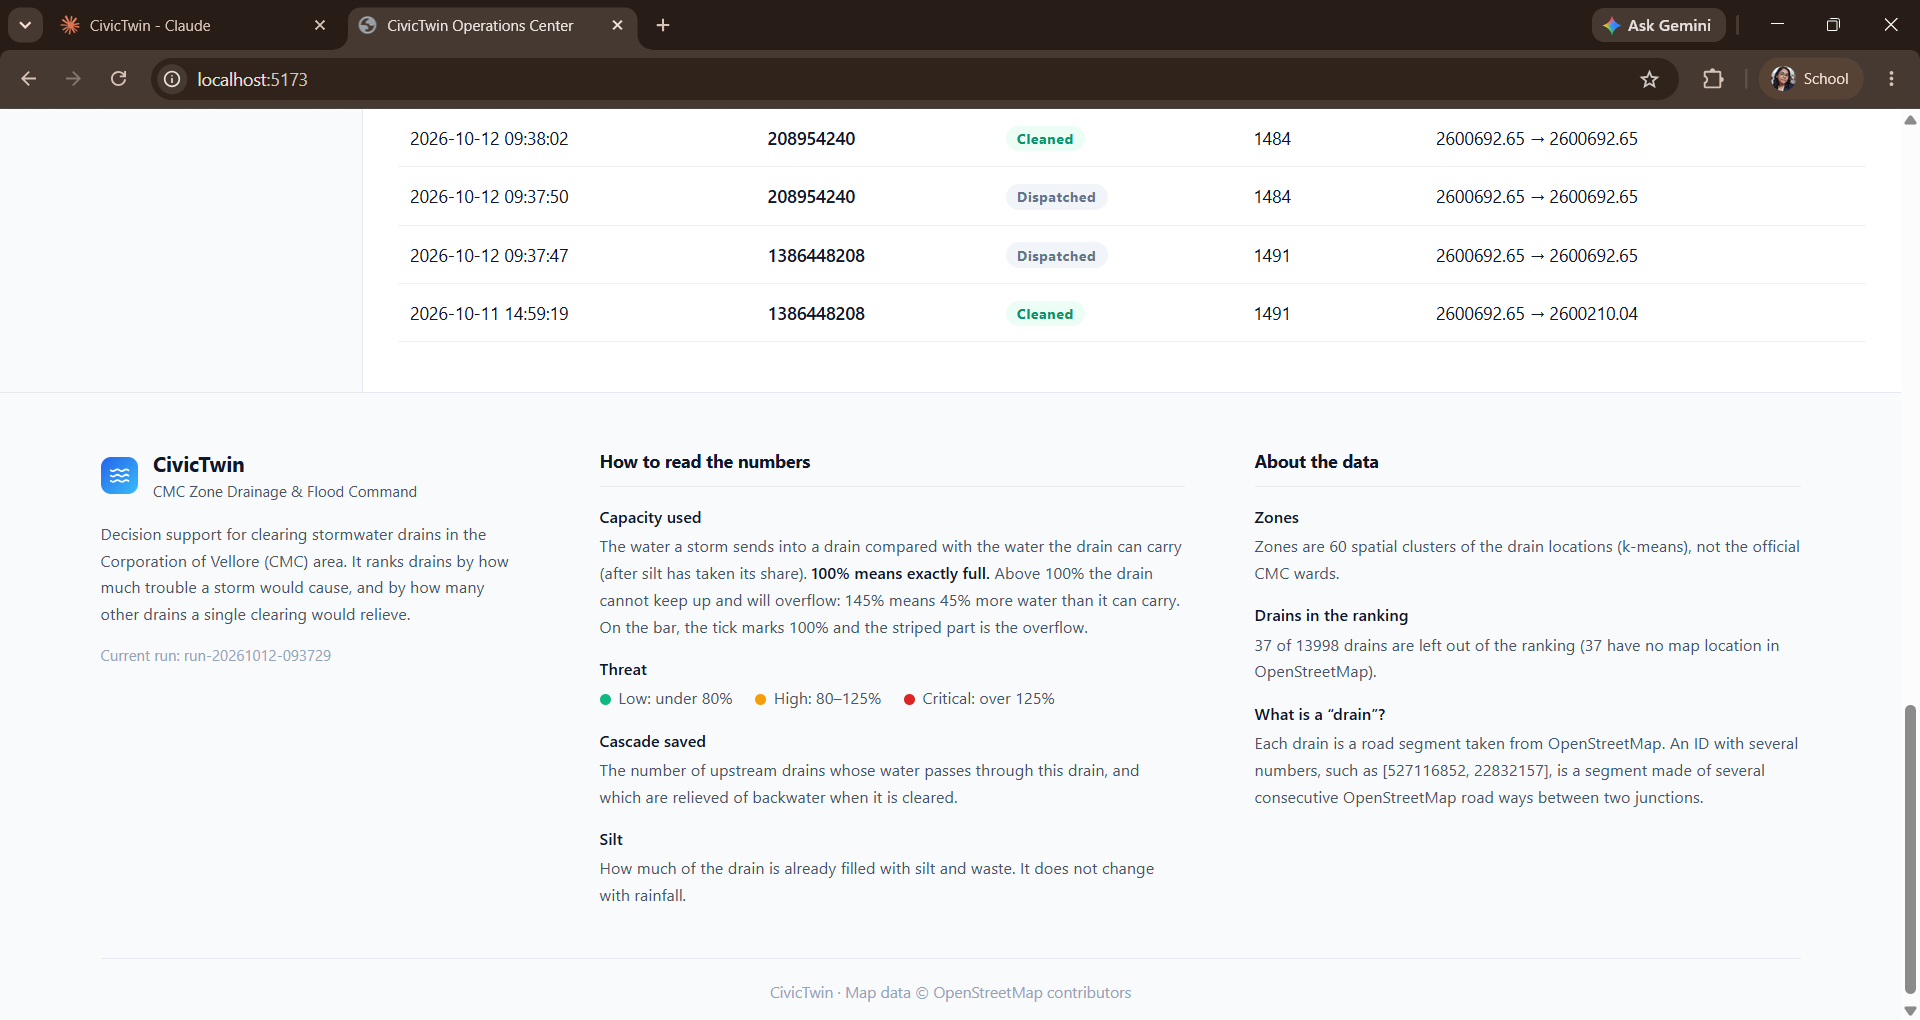
\includegraphics[width=0.98\textwidth]{figures/ui_logs_and_guide.png}
\caption*{Fig. A.3 Activity Audit Log and Administrative Metric Interpretation Guidelines}
\end{figure}
